\documentclass{prova}

\usepackage{amsmath}
\usepackage{amsfonts}

\setlength{\textheight}{25cm}

\renewcommand{\sin}{\,\mbox{sen}\,}
\newcommand{\ds}{\displaystyle}

\professor{Prof.\@ Adriano Barbosa}
\disciplina{C\'alculo de V\'arias Vari\'aveis}
\avaliacao{P2}
\curso{Matem\'atica}
\data{19/04/2023}

\begin{document}
	\cabecalho{5}  % o numero 5 indica a qnt de quadros na tabela de nota

    \textbf{Todas as respostas devem ser justificadas.}

    \begin{questionario}
        \q{Calcule a integral dupla $\ds\iint_R y\sin(xy)\ dA$,
           $R=[1,2]\times [0,\pi]$.}
        \q{Esboce ou descreva a regi\~ao cuja \'area \'e dada pela integral
           $\ds\int_{\pi/4}^{3\pi/4} \int_1^2 r\ dr\,d\theta$ e calcule-a.}
        \q{Calcule a integral $\ds\iint_D \sin(y^2)\ dA$, $D=\{(x,y)\ |\ 0\le
           x\le 1, x\le y\le 1\}$.}
        \q{}
            \begin{questionario}
                \qq{Escreva a integral tripla de uma fun\c{c}\~ao cont\'{\i}nua $f(x,y,z)$
                    sobre o s\'olido abaixo determinando seus limites de
                    integra\c{c}\~ao.}
                \qq{Calcule o volume do s\'olido utilizando a integral tripla
                    encontrada no item anterior.}
                \begin{figure}[h]
                    \centering
                    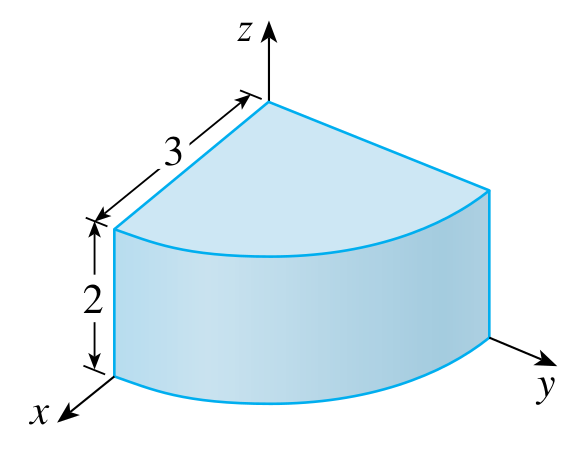
\includegraphics[width=0.3\textwidth]{fig1.png}
                \end{figure}
            \end{questionario}
        \q{Calcule $\ds\iiint_E x^2+y^2\ dV$, onde $E$ est\'a entre as
           superf\'{\i}cies $x^2+y^2+z^2=4$ e $x^2+y^2+z^2=9$.}
    \end{questionario}
\end{document}
